\chapter{ Introducción}
Breve introducción donde se explica la motivación de dicho trabajo, como ha sido planteado en el tiempo, sus objetivos principales y secundarios y la estructura que tiene cada uno de los capítulos que forman la memoria.
\section{Motivación}
Cierto es que el uso de la informática y la tecnología está en auge en nuestra sociedad. Esto está llegando no solo a facilitar nuestra vida cotidiana, sino también a apoyar y beneficiar la aplicación de la medicina y la salud. Por ejemplo, la electromiografía (EMG) es de gran utilidad para analizar el comportamiento y la activación de las unidades motoras (Figura \ref{fig:motoneurona}) a la hora de realizar cierta actividad física. Esto, junto con la multitud de características que se pueden extraer de las señales EMG adquiridas, hace que se puedan realizar multitud de estudios para analizar el rendimiento y patologías de pacientes. Haciendo uso de un buen diseño e implementación se puede llegar a obtener un sistema de tiempo real donde se pueda realizar el diagnostico en el mismo momento de la actividad física y poder analizar los diferentes datos tomados \cite{konrad2005abc}.

\begin{figure}[ht]
\centering
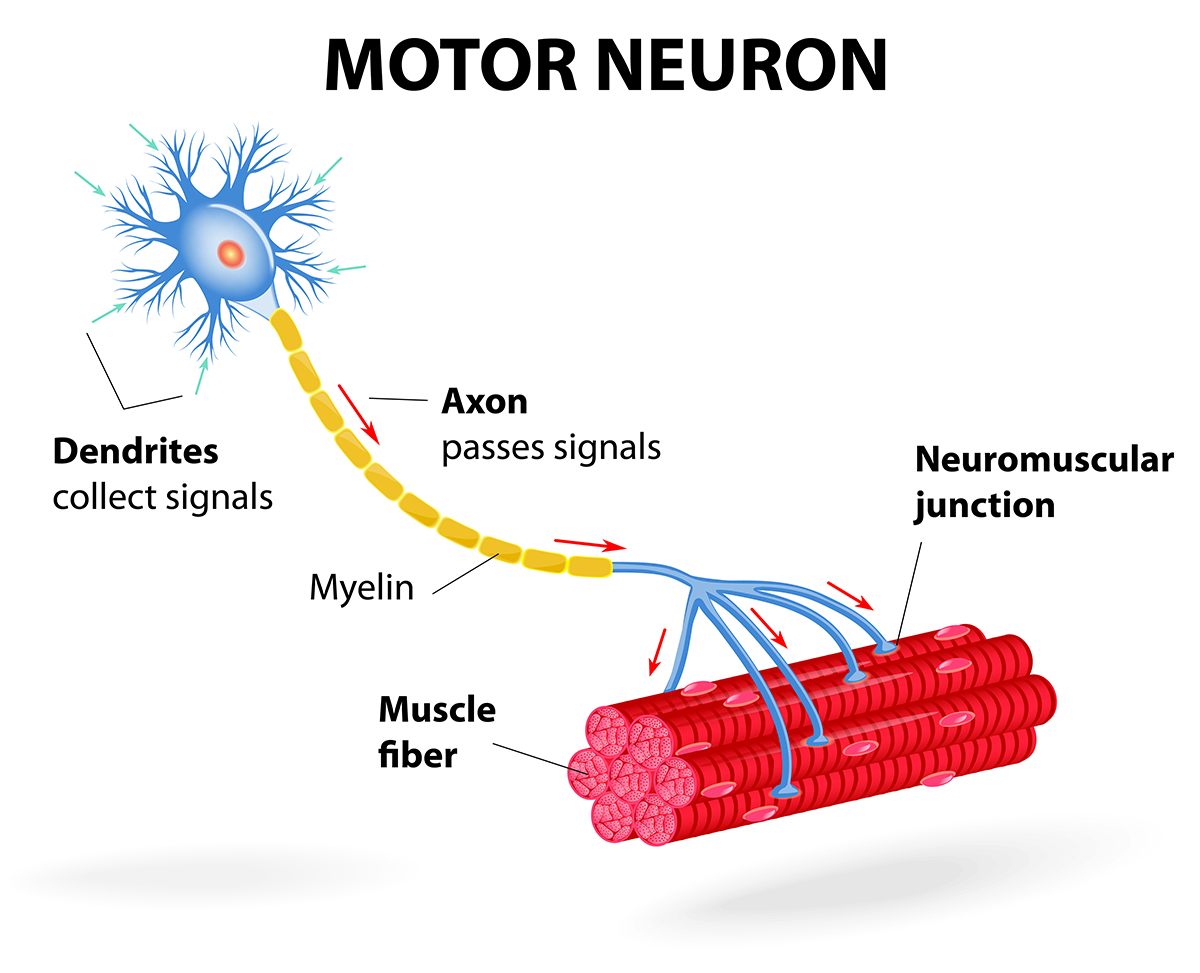
\includegraphics[scale=0.25]{imagenes/motoneurona.jpg}
\vspace{-1.0cm}
\caption{ Ejemplo de motoneurona \cite{motoneurona1}}
\label{fig:motoneurona}
\end{figure}
Existe un gran número de deportistas que cuando entrenan hacen todo lo posible para evitar la fatiga muscular. Por ejemplo, sería el caso de atletas que practican powerlifting o halterofilia, donde el objetivo es levantar el mayor peso posible en una sola repetición. Estos atletas evitan los entrenamientos bajo fatiga debido a que cuando entrenan bajo fatiga no consiguen un rendimiento óptimo. Esto se debe a que cuando se entrena bajo fatiga, el esfuerzo que se tiene que realizar es mucho mayor, así como la probabilidad de lesión. Además aunque el esfuerzo realizado sea mayor, no implica que la fuerza ejercida sobre la carga levantada también lo sea, ya que no se están reclutando tantas fibras musculares.

El aumento del esfuerzo realizado y la mayor probabilidad de lesión se deben a que cuando el sistema nervioso central entra en fatiga no recluta tantas unidades motoras y por ende, no existe tanta activación muscular. Como sabemos la musculatura complementa al sistema óseo y por lo tanto un déficit en la implicación de algún músculo debido a la fatiga hará que se incremente la posibilidad de lesión en articulaciones y ligamentos. Por ejemplo, en algunas lesiones de rodilla como la rotura del ligamento cruzado anterior, se produce una compensación entre cuádriceps e isquiotibial. Una entrada en fatiga de ambos músculos, quitaría mucha estabilidad a la rodilla y aumentaría el daño en el ligamento. Si el ligamento, en lugar de sufrir una rotura total, solo estuviese roto parcialmente, es decir, una lesión más leve, lo que se conseguiría entrenando bajo fatiga sería incrementar la lesión.
Todo esto se explica con mayor detalle en el capítulo \ref{analisis} .

En este proyecto se ha tratado de desarrollar una herramienta que ayuda a los fisioterapeutas a la hora de detectar la fatiga muscular. Con ello se pretende dotar al fisioterapeuta de la suficiente información como para determinar que músculo ha experimentado dicha fatiga y así poder estudiar si se ha producido una compensación muscular a la hora de la ejecución de una sentadilla y determinar si hay una lesión en dicha rodilla. Además, como se ha comentado en párrafos anteriores, en multitud de sistemas de entrenamientos basados en fuerza, está desaconsejado el entreno bajo fatiga, ya que se considera contraproducente. Esto implica otro posible uso de dicho sistema, y es que podría ser utilizado por atletas expertos, en entrenamientos de fuerza como powerlifting o halterofilia para detectar la fatiga en el momento del entreno y cortar la serie para descansar y no tener un entreno contraproducente. 

Para determinar la fatiga en este proyecto, se ha puesto la condición de que cuando un atleta está realizando una serie de sentadillas y su velocidad de ejecución decae un 20 por ciento, es un indicativo de fatiga. Esta condición se debe de cumplir en dos repeticiones seguidas, para así determinar una fatiga más representativa. La condición de la caída de velocidad fue propuesta por el fisioterapeuta de la empresa encargada de la toma de datos, mDurance \cite{mDurance}, además de ser bastante utilizada en el mundo del deporte \cite{fernandezpropuesta}.

Cabe destacar que este proyecto ha sido llevado a cabo con la colaboración de mDurance \cite{mDurance}, una empresa especializada en electromiografía y que ha sido la encargada de aportar los datos para realizar el estudio de los diferentes clasificadores. Han aportado datos de electromiografía sobre los músculos vasto medial y recto femoral de ambas extremidades inferiores a la hora de realizar sentadillas.


\section{Planteamiento del trabajo}
Para solucionar el problema de la detección de la fatiga muscular y también poder determinar si existe o no compensación muscular y por ende una lesión en la rodilla se pretende desarrollar un modelo que clasifique las señales de EMG recibidas entre fatiga y no fatiga. 

Para ello, el desarrollo del modelo consta de tres fases principales. Una primera fase de extracción de características de la señal EMG, tales como RMS, MAV, MDF, etc. En el capítulo \ref{cap6} se comentan todas las características estudiadas junto con su definición. Una segunda fase de selección de las características más representativas de la fatiga, para quedarnos con la menor cantidad posible y así obtener un clasificador más eficiente y rápido. Finalmente una fase de clasificación donde se probarán diferentes clasificadores para finalmente quedarnos con el que mejor prestaciones tenga para dicho problema. 
Con dicho clasificador se podría clasificar las señales EMG recibidas en tiempo real para determinar si la persona que está realizando las repeticiones de sentadillas ha sufrido fatiga y en el momento en el que la ha sufrido. 

Con esta herramienta los fisioterapeutas y médicos podrían realizar pruebas a sus pacientes para luego llegar a ciertas conclusiones. Todo esto sin la necesidad de tener una maquinaria muy compleja, ya que una vez implementado y entrenado el clasificador, no sería necesario medir la velocidad de ejecución de las series de los pacientes a los que se va a realizar la prueba.

Por último comentar que para la realización de este proyecto han sido necesarios datos reales, tomados y filtrados por la empresa especializada en electromiografía mDurance. Además de los datos de las diferentes señales de electromiografía, fue necesario una medición de la velocidad de cada repetición para así, al tener la velocidad de cada repetición poder estimar que sujetos experimentaron fatiga y utilizar dichos datos para entrenar y analizar el rendimiento de los diferentes clasificadores.
\section{Objetivos\label{objetivos}}

Como consecuencia de lo planteado anteriormente el objetivo general sería obtener un clasificador que reciba los datos de la señal EMG y clasifique en tiempo real entre fatiga y no fatiga. Esto servirá para detectar la fatiga en tiempo de ejecución con una herramienta muy sencilla y una vez entrenado el modelo, no sería necesario la utilización de un velocímetro para medir la velocidad de ejecución de cada repetición y estimar la fatiga. Esto se debe a que nuestro modelo, una vez entrenado, solo por el análisis de las señales será capaz de catalogar las señales de EMG entre fatiga y no fatiga. Además una vez clasificadas las señales EMG, el personal especializado para ello podrá determinar si existe compensación entre músculos implicados en el movimiento normal de la rodilla y determinar si existe algún tipo de lesión.

Con respecto a los objetivos específicos, están muy relacionados con las tres fases comentadas anteriormente.
\begin{itemize}
\item Analizar y procesar las señales brutas de EMG.
\item Analizar la velocidad registrada de cada sujeto.
\item Estimar la fatiga de cada uno de los sujetos.
\item Extraer características de las señales de EMG.
\item Crear los archivos de entrenamiento-testeo.
\item Seleccionar las características más útiles para el modelo final.
\item Clasificar las señales de EMG. 
\item Validar el rendimiento de los modelos.
\end{itemize}
\section{Estructura del trabajo}
En este capítulo 1, todo lo comentado es una breve introducción al problema a resolver y a la realización del proyecto. Más adelante se explicarán con más detalle las pautas que se han seguido para el desarrollo del proyecto.

En el capítulo 2 se comenta el estado del arte donde se hará un análisis en profundidad del problema en cuestión, de toda la tecnología que abarca y su posible aplicación en la actualidad.


En el capítulo 3 se comenta la planificación llevada a cabo para la realización del proyecto, así como el coste económico final y parcial.

En el capítulo 4 se hace un análisis del problema tratado. La fatiga muscular, como afecta al sistema nervioso y los problemas musculares asociados a las lesiones de rodilla.

En el capítulo 5 se realiza un diseño de todas las fases realizadas para el proyecto. Consta de un gran número de esquemas donde se explica el funcionamiento de los algoritmos utilizados y los tipos de archivos de entrenamiento-testeo implementados.

El capítulo 6 es el dedicado a la implementación. En él se puede encontrar el código asociado al desarrollo del proyecto.

El capitulo 7 está dedicado a la sección de pruebas. En él se pueden encontrar todos los resultados de los clasificadores diseñados y una opinión personal sobre sus rendimientos.

Por último, el capítulo 8 es el dedicado a las conclusiones y trabajos futuros. En él se comenta si se han cumplido los objetivos de este proyecto y consejos para una futura aplicación junto a una herramienta de electromiografía.


